\documentclass[12pt]{article}
\usepackage{graphicx}
\usepackage[utf8]{inputenc}
\usepackage{makecell}
\usepackage[margin=1in]{geometry}
\usepackage[T1]{fontenc}
\usepackage{mathptmx}
\usepackage[normalem]{ulem}
\usepackage{placeins}

\renewcommand\theadalign{bc}
\renewcommand\theadfont{\bfseries}
\renewcommand\theadgape{\Gape[4pt]}
\renewcommand\cellgape{\Gape[4pt]}
\graphicspath{ {./images/} }
\usepackage[
backend=biber,
style=numeric,
sorting=none,
citestyle=ieee
]{biblatex}

\addbibresource{bibliography.bib}

%opening
\title{Software Design Description for Project Name }
\author{
Nour Ahmed, Nour El Hoda Hisham, Mariam Hesham, Samiha Hesham ,Sandra Fares\\
Supervised by: Eng. Lobna Mostafa,  Dr. Islam Tharwat
}
\begin{document}
\maketitle

\begin{table}[htbp]
\caption{Document version history}
\begin{center}
\begin{tabular}{|c|c|l|}
\hline
\thead{Version}    & \thead{Date} & \thead{Reason for Change}  \\ \hline
1.0 & 25-Jan-2021   & \makecell[l]{SDD first version’s description are defined.}   \\ \hline
1.1 & 2-Feb-2021   & \makecell[l]{Added Sequence Diagram.} \\ \hline
1.3 & 5-Feb-2021   & \makecell[l]{Requirement Matrix updated.} \\
\hline
\end{tabular}
\end{center}
\end{table}

\begin{table}[htbp]
\begin{tabular}{cc}
\thead{GitHub:}    & {https://github.com/SandraFW/intelligent-Surveillance-for-smart-cities}   
\end{tabular}
\end{table}

\pagebreak
\tableofcontents
\pagebreak

\begin{abstract}
Add your project abstract here.
(Word Limit 150)
\end{abstract}

\section{Introduction}

\subsection{Purpose}
The purpose of the software design document (SDD) is to present the project ” Intelligent Surveillance for smart cities” thoroughly. SSD illustrates the framework and system design architecture of the proposed system. Moreover, the document provides a fully detailed system overview and scope besides stating the main objective of the system. The SDD document is considered a significant guide for the project team members and for the customer to be fully aware of the project. Also, for the developers to improve and develop the system in the future.

\subsection{Scope}

The scope of the software design document (SDD) is to describe the project ” Intelligent Surveillance for smart cities” in detail. The SDD provides the main design of the data and viewpoints to communicate to key design stakeholders. Also, it states the main objective of the system with a well-studied timeline. Besides, the algorithms and human Interface design that utilized in the project. Moreover, the states of the functional requirements of the system.

\subsection{Overview}
The software design document (SDD) presents the overall system architecture in addition to design patterns, data models, data structures, algorithms, and design viewpoints. Moreover to the human interface design to know how to utilize the provided services correctly. The software design document is structured as follows.

 Section I introduces the document by defining its purpose, scope, and overview. In addition to the audience that the document is intended for. Section II presents the system thoroughly by illustrating the system overview and describing the functionality of the whole system. In addition to the system scope and brief description of system main features and boundaries. Moreover, it states the main objective of the system with the project plan. Section III illustrates the design viewpoints of the system. Section Iv presents the data design for the system. It explains the information related to the data in the system and how it is stored. In addition to the thorough description of the dataset and database utilized in the system. Section V presenting the human interface design for the system. Section VI describes the requirements matrix that clarifies the status of the functional requirements mentioned in the SRS. Section VII stating the appendices that could help in well understanding the document.

\subsection{Intended audience}

1)	Dr. Islam Tharwat

2)	Eng. Lobna Shaheen

3)	Nour Ahmed Ghoneim (Team Leader)

4)	Nour Elhoda Hesham

5)	Samiha Hesham

6)	Sandra Wardkhan

7)	Mariam Hesham



\subsection{Reference Material}
We have done a  systematic review, as well as a review paper, which was sent to SSIC 2021,(3rd International Conference on Smart Systems: Innovations in Computing), SRS which is mainly talking about how to use edge-fog model and  Proposal.

\begin{figure}[htbp]
\centering
\includegraphics[width=0.9\linewidth]{reference1.png}
\caption{Systematic Review}
\label{archdsgn}
\end{figure}
\FloatBarrier

\begin{figure}[htbp]
\centering
\includegraphics[width=0.9\linewidth]{reference2.png}
\caption{Proposal}
\label{archdsgn}
\end{figure}
\FloatBarrier

\begin{figure}[htbp]
\centering
\includegraphics[width=0.9\linewidth]{reference3.png}
\caption{SRS}
\label{archdsgn}
\end{figure}
\FloatBarrier

\subsection{Definitions and Acronyms}

\begin{table}[htbp]
\begin{tabular}{|p{0.35\textwidth}|p{0.85\textwidth}|}
\hline
\multicolumn{1}{|c|}{\textbf{Term}} & \multicolumn{1}{c|}{\textbf{Definition}}                                                                                              \\ \hline
EFISS                      & \begin{tabular}[c]{@{}l@{}}Edge Fog intelligent surveillance system.\end{tabular} \\ \hline
Graphical User Interface (GUI)      & \begin{tabular}[c]{@{}l@{}}is a form of user interface that allows user to interact with electronic devices\\ through graphical icons and audio indicator .\end{tabular}                  \\ \hline

Design rationale                      & \begin{tabular}[c]{@{}l@{}}Information capturing the reasoning of the designer that \\led to the system as designed, including design options, \\trade-offs considered, decisions made, \\and the justifications of those
decisions. .\end{tabular} \\ \hline

\end{tabular}
\end{table}
 
\section{System Overview}


\subsection{System Scope}

\begin{enumerate}
\item Fog/Edge computing-based surveillance system to monitor the whole city 24/7.

\item Privacy assurance by blurring people’s faces to secure their exposed identity in the video.
\item Scalability system to handle such massive data generated from surveillance cameras and sensors.
\item Efficient image processing techniques for certain failures in the edge cameras that impacts the usefulness of the video streams.
\item Dispatch crime details (i.e., video and location of the event, criminal’s face) and giving alert to the nearest competent authority.

\item Providing efficient real-time tracking for the criminal in case of detecting an incident.

\end{enumerate} 

\subsection{System objectives}
\begin{enumerate}


\item The system will be able to detect the action occurred accurately.

\item The system should apply blurring method for normal citizen’s bio-metrics in order to enhance privacy in surveillance system.
\item The system should send alert if any failure is detected in the cameras in order to help the maintenance team to solve the problem.
\item The system will send alert message when anomaly behaviour is detected using the fog nodes in the architecture system.

\item The system will filter the incident using video splitting technique in order to be saved and sent to the cloud to save storage.
\item The system will be able to predict the event before occurring in order to prevent it and avoid tragic situations.
\item The system should provide face recognition feature for the kidnapper and the victim to get their information.
 \end{enumerate}
 
\subsection {System Timeline}

\begin{table}[htbp]
\centering
\caption{ISS time plan}
\label{tab:Time Plan}
\begin{tabular}{|l|l|l|l|l|}
\hline
Id & Task               & Start Date & Number of Days & Team Member \\ \hline
1  & Collect Dataset    & 12/10/2020 & 10             & X, Y        \\ \hline
2  & Work on GUI        & 12/21/2020 & 15             & Z, Y        \\ \hline
3  & Pre-Processing     & 12/21/2020 & 5              & X           \\ \hline
4  & Feature Extraction & 12/26/2020 & 5              & X, Z, Y     \\ \hline
5  & Classification     & 12/31/2020 & 10             & Z           \\ \hline
6  & Writing Paper      & 01/05/2021 & 30             & X, Z, Y     \\ \hline
7  & Experiments        & 01/10/2021 & 20             & X, Z, Y     \\ \hline
\end{tabular}
\end{table}

\begin{figure}[htbp]
\centering
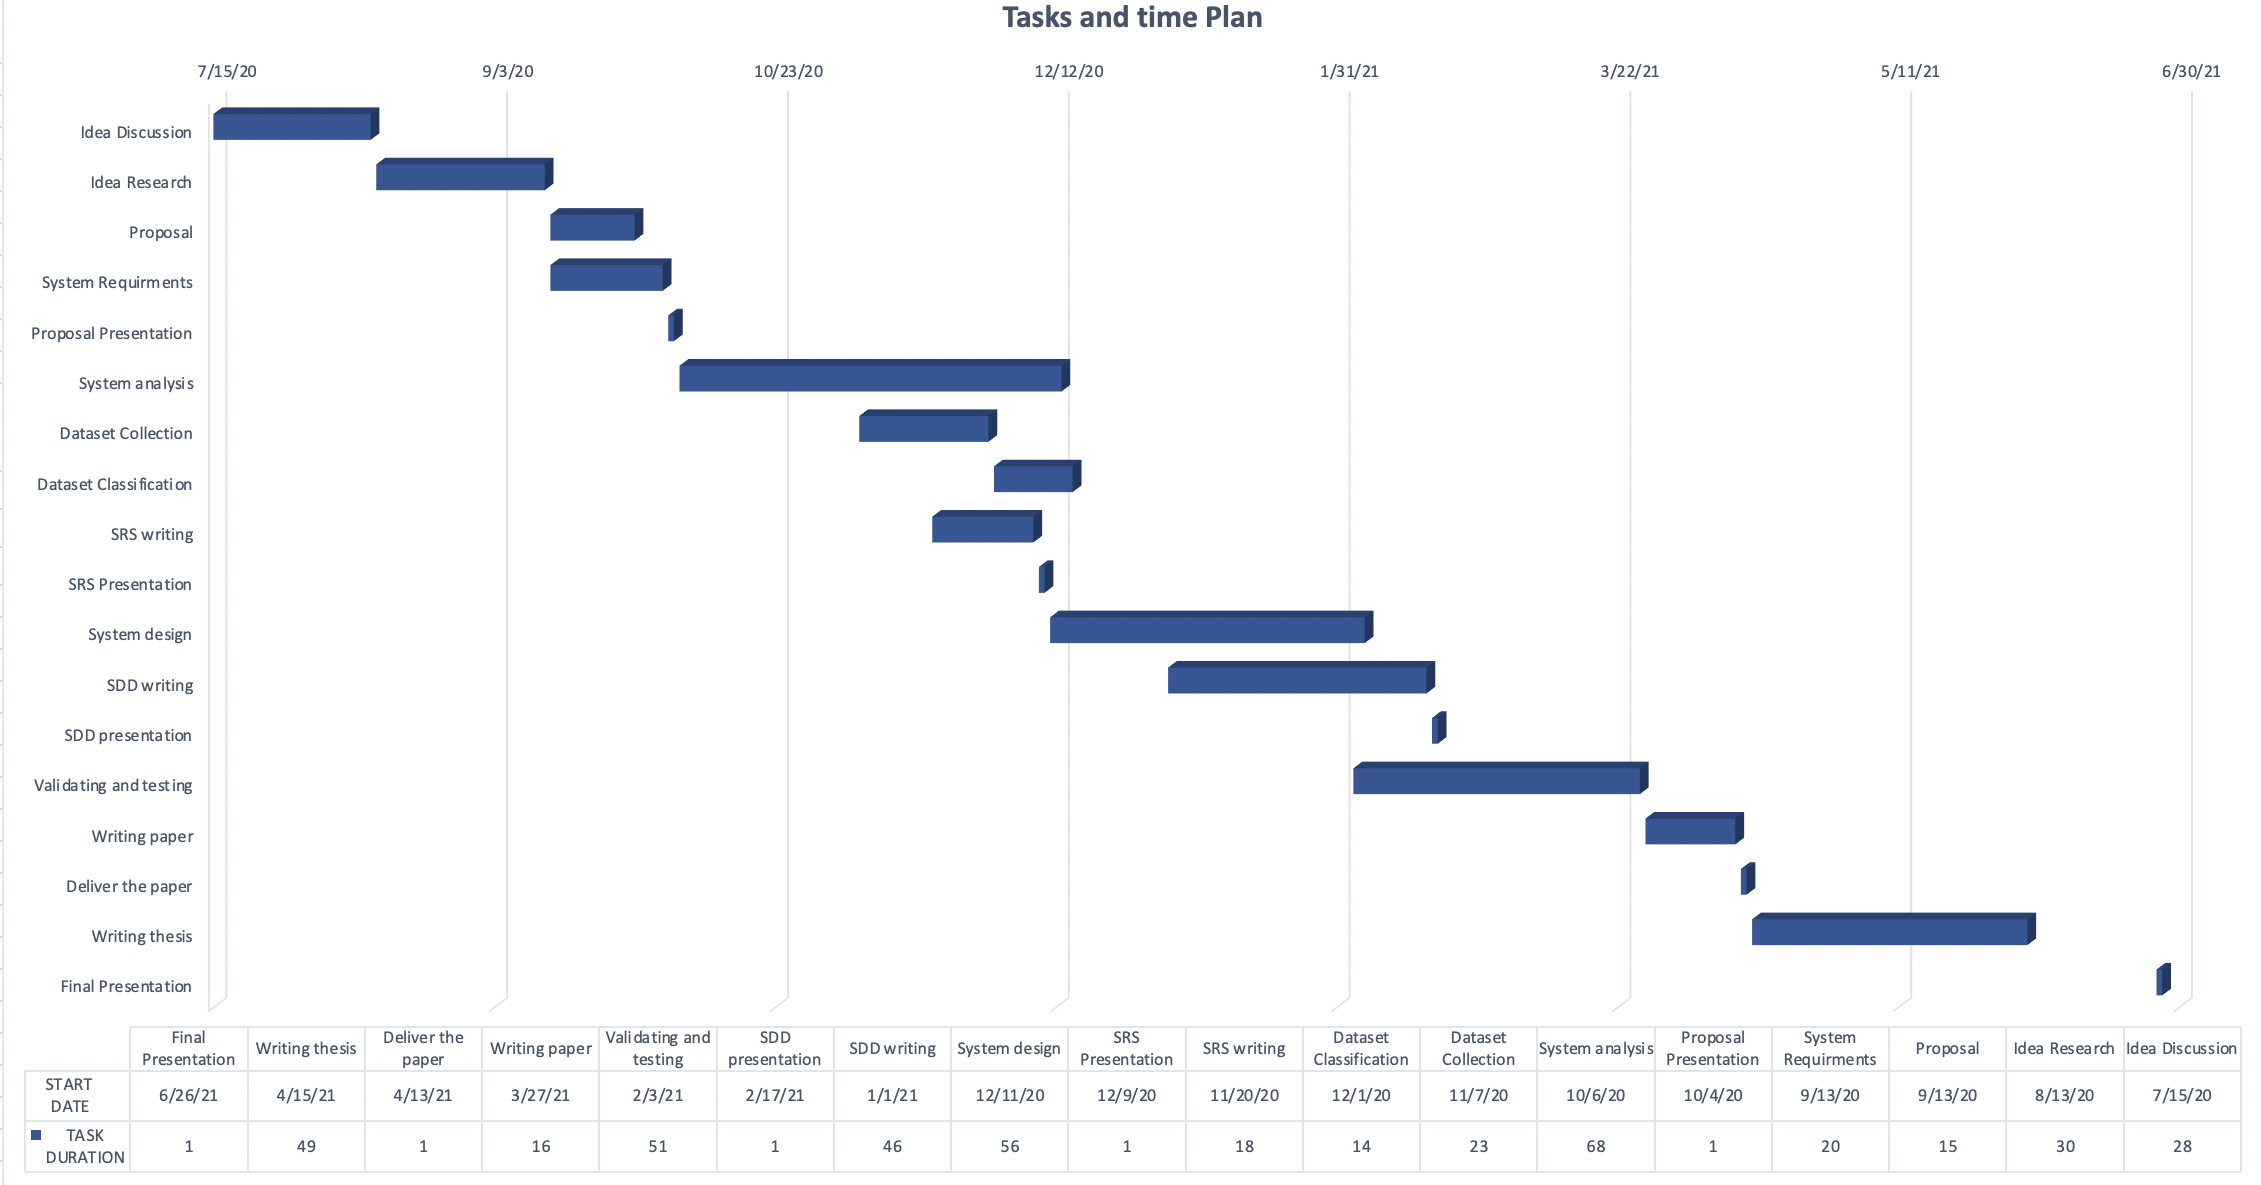
\includegraphics[width=\linewidth]{Taskplan.PNG}
\caption{ISS GANTT Chart}
\label{fig:GANTT Chart}
\end{figure}

\clearpage
\section{Design viewpoints} 
\subsection{ Context viewpoint}
The intelligent surveillance system monitors smart city streets to assists the police units to get notified of any incident that occurs to take quick action against it using the three computing layers Edge, Fog and cloud. Our proposed system aims to provide a high level of safety to the citizens. Therefore the system captures the pedestrians to collect data throughout the day. The collected data are processed to detect any failure in the surveillance cameras or whenever an abnormal activity occurs, it captures the incident, then identifies whether it is a crime or not; if it is, the system identifies the criminal and forwards the collected information to the police unit to take the proper action and helps them track the criminal.

\begin{figure}[htbp]
\centering
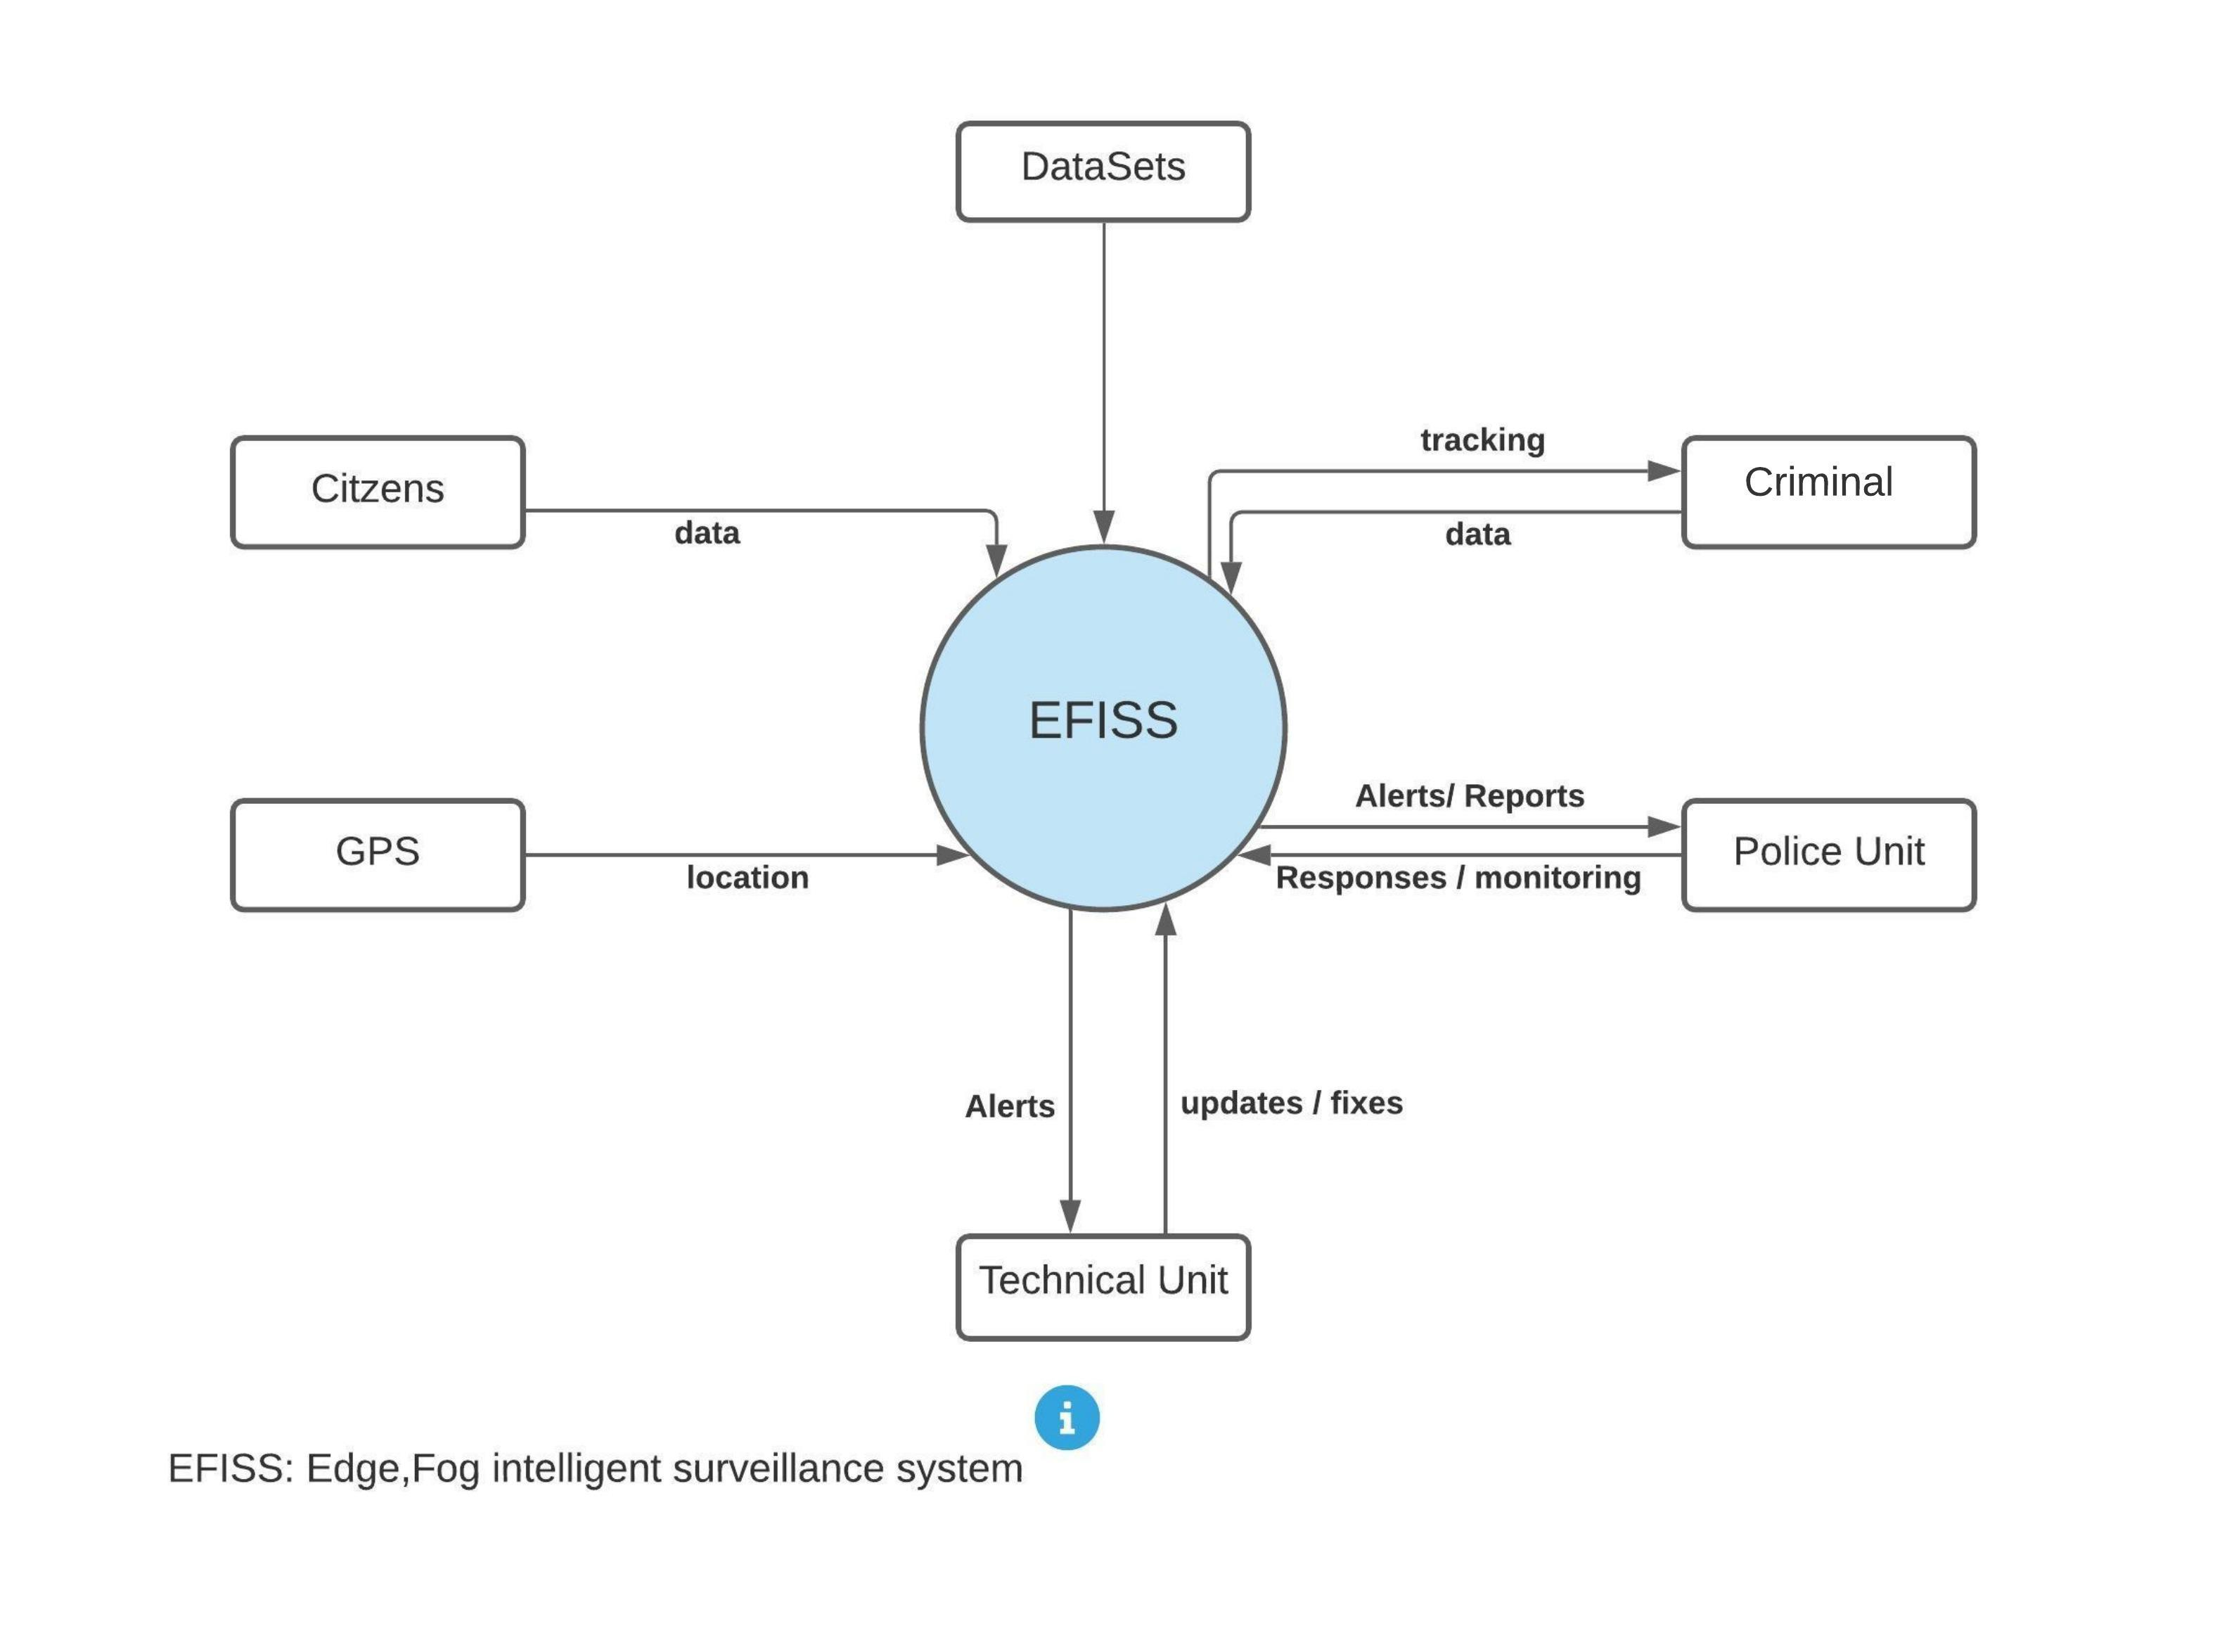
\includegraphics[width=0.8\linewidth]{contextdiagram.jpeg}
\caption{Context Diagram for the Edge Fog intelligent surveillance system}
\label{fig:ctx}
\end{figure}
\FloatBarrier

\begin{figure}[htbp]
\centering
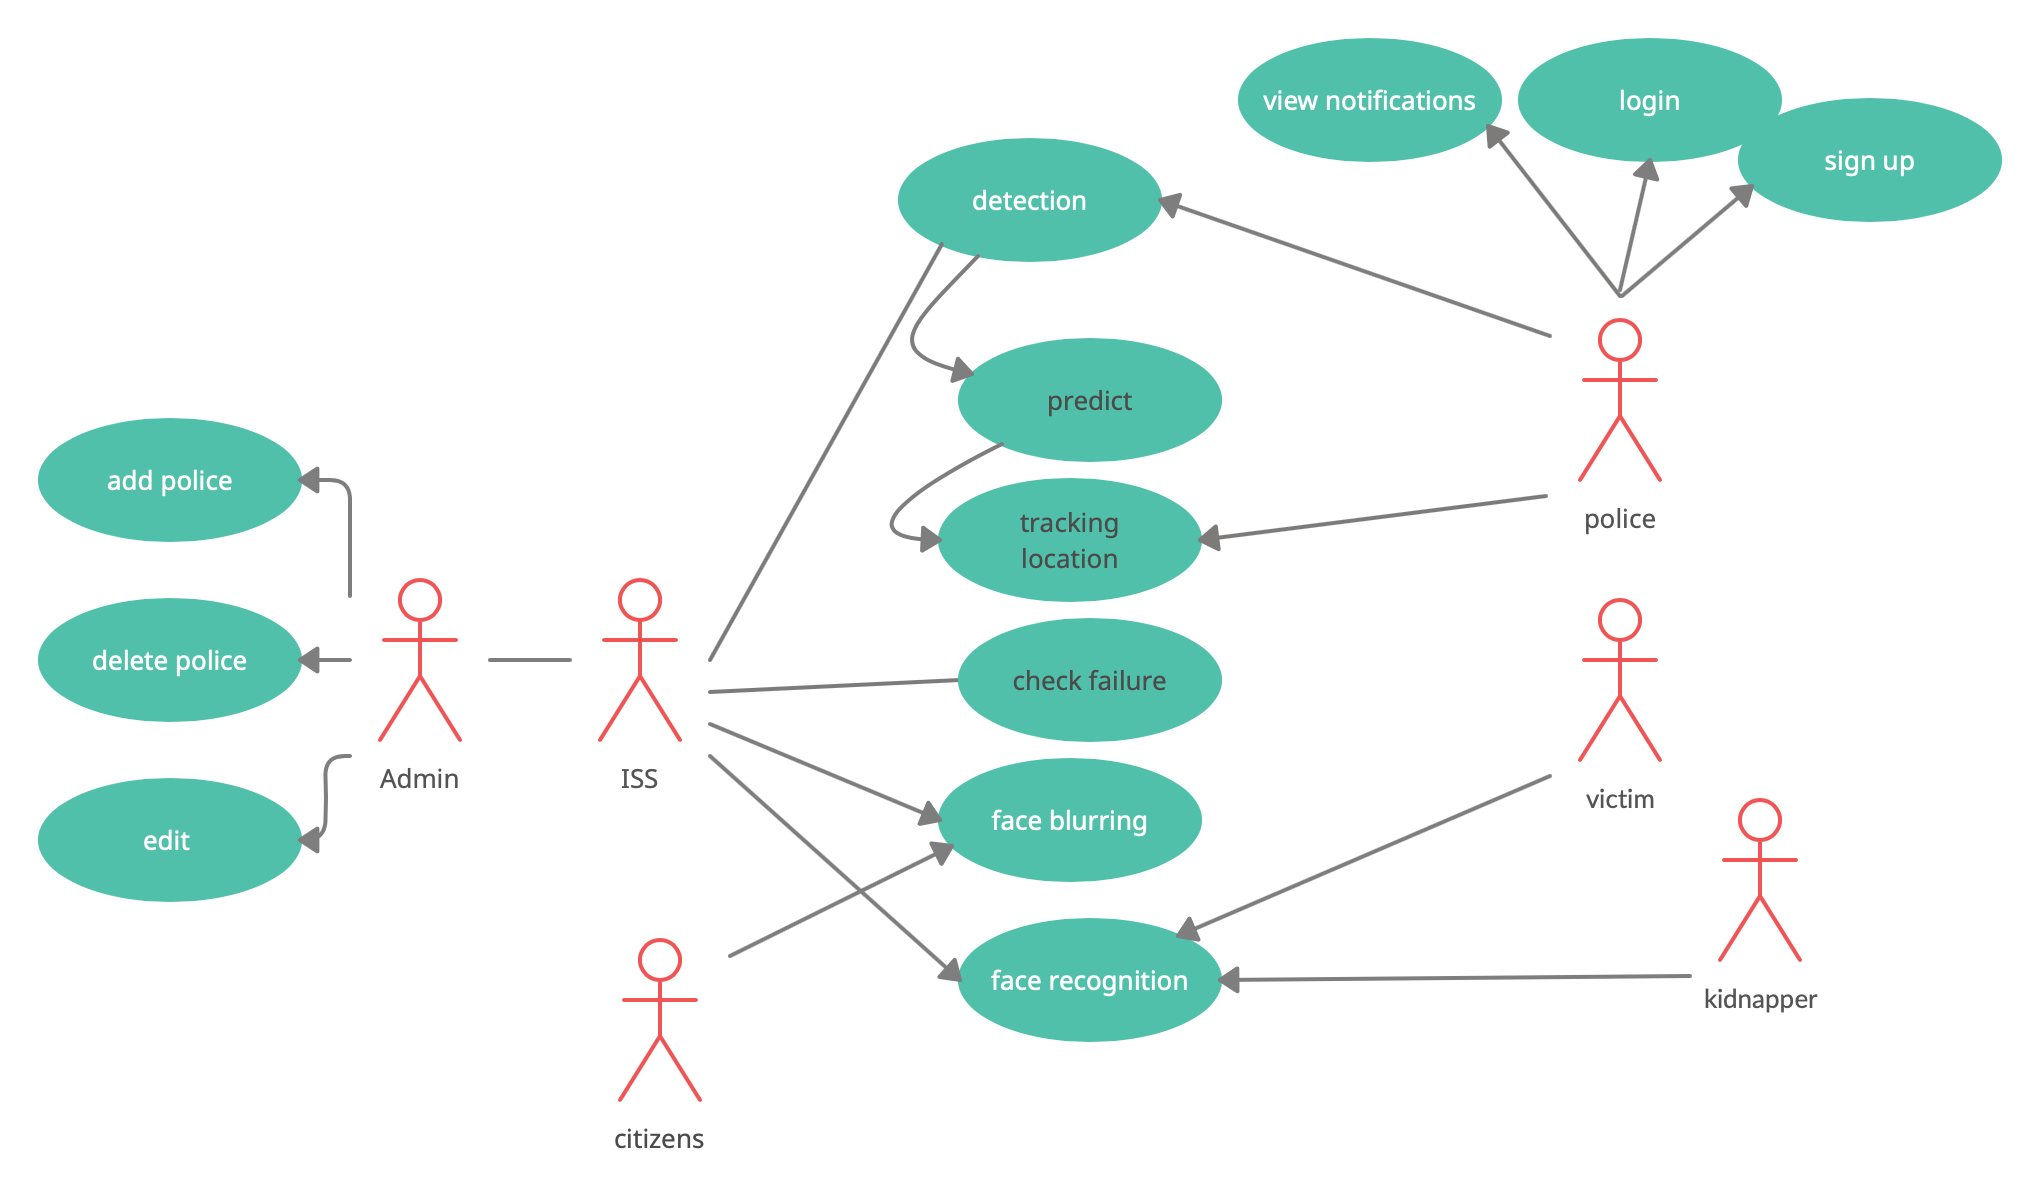
\includegraphics[width=0.9\linewidth]{survillienceusecase.png}
\caption{Use Case Diagram Example}
\label{fig:ucase}
\end{figure}
\FloatBarrier
\subsection{Composition viewpoint}\label{ss-comp}

Our system is composed of three layers Edge, Fog, and cloud layers; Each of them has responsibilities, and they communicate together through a stable network to provide the user at the end the needed result.
\begin{itemize}
\item Edge Layer: The first layer in our system is the surveillance cameras fixed within the smart street lights. Those cameras are responsible for capturing the pedestrians throughout the day and using a crime detection algorithm whenever any abnormal actions are recognized the video stream is transferred to our second layer; and if everything is normal, the videos are being stored on the camera's local storage and then sent to the cloud when the network is free. Also, we consider any failure in cameras using a failure detection algorithm to avoid any blurry recording, green or black videos being recorded. Finally, there is a comparing algorithm that helps tracking wanted criminals whenever detected in any street the authorities are informed.
\item Fog Layer: The second layer in our system, This layer is divided into two sub-layers; the first depends on connected vehicles near the incident and the second is smart traffic light which works as gateways.
\subitem The vehicles layer: It is responsible for extracting more features from the video stream to be more sure about the incident and summarize it into an image using a special algorithm for further processing in the second fog sub-layer.
\subitem The smart traffic light: It is responsible for the final processing of the incident using a deep learning algorithm; to ensure the incident, classify it and send it to the cloud layer the final layer. Also, an image processing deblurring algorithm is applied for face detection. then the criminal face image is sent back to the edge nodes.
\item Cloud Layer: The final layer; is responsible for triggering the alarms and send notifications for our end users, and backup all the incident data sent. Also, it is used for archiving all the videos captured throughout the day.
\item All the layers should communicate together using a stable wireless network provided in the smart city.
\end{itemize} 

\begin{figure}[htbp]
\centering
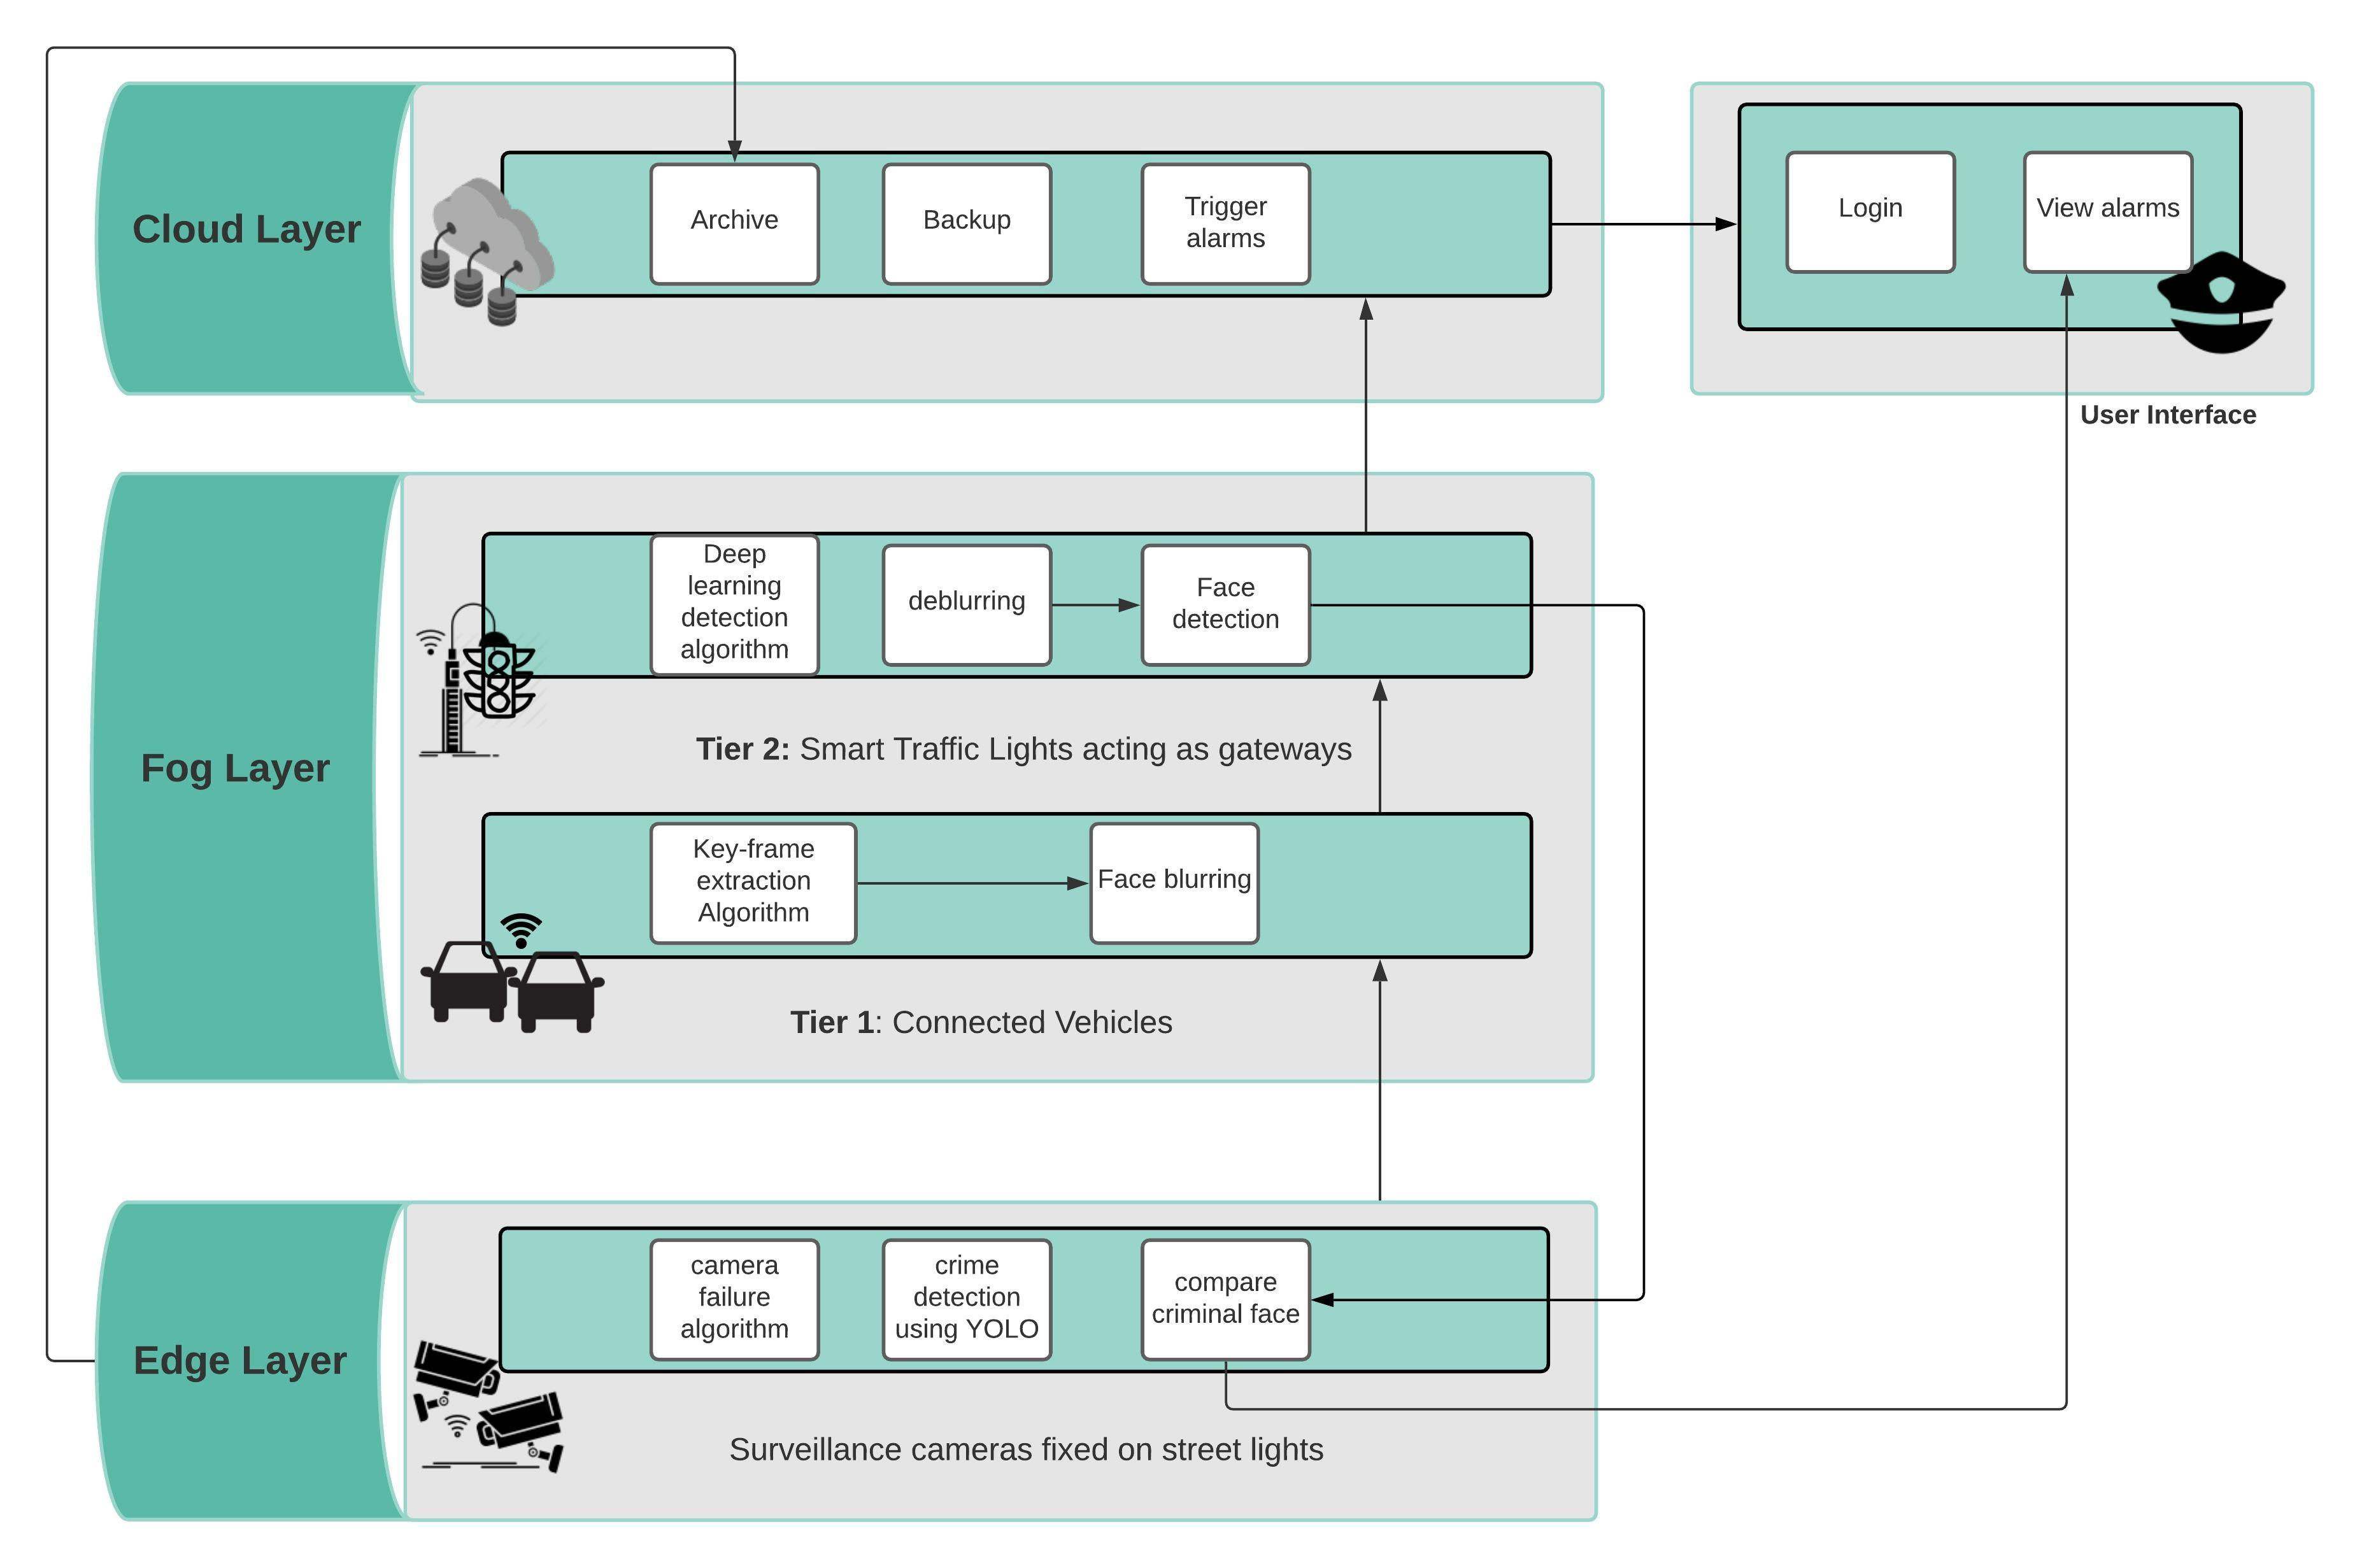
\includegraphics[width=0.9\linewidth]{arch.jpeg}
\caption{Architectural Design Diagram }
\label{archdsgn}
\end{figure}
\FloatBarrier
\textbf{Design concerns:}
Main design concerns are focused on robust and efficient communication between each computing layer. We put into consideration the computational power of devices used in each layer to be compatible with the functions deployed to them. performance of the functions, liable deep learning operation results, and avoiding false-negative detection also was of the main concerns to avoid false alarms.Finally, the system should follow ethics and protects the privacy of the citizens.

\subsubsection{Design Rationale}
Various architectures have been introduced in the field of real-time video surveillance.
\begin{itemize}
\item Cloud Computing: At first, systems were implemented using only a cloud computing layer; But they were expensive, relatively slow to perform real-time video surveillance, and there was consistently heavy traffic on the network. 
\item Edge or Fog layers and cloud Computing : Therefore, they started adding fog layers or edge layers individually, where the performance was enhanced; but it was introduced for smaller areas as smart homes, also the devices used needed high computational power or less powerful functions were used.
\end{itemize}
\newline  So, We built our architecture that comprises all three layers to get maximum advantages from each layer; to easily monitor the whole smart city. Each layer performs specific functions either simple image processing or deep learning algorithms, therefore most of the false alarms were reduced; those functions were chosen to be deployed according to each layer's components' computational power and to efficiently serve the proper flow of the system. Then each layer communicates with others through a stable network to forward and process the results in case of detecting an incident only; thus the network traffic was reduced. And finally notifying our end users of those incidents efficiently.
\FloatBarrier
\subsection{Logical viewpoint}

\subsubsection{Class Diagram}
 \FloatBarrier
\begin{figure}[htbp]
\centering
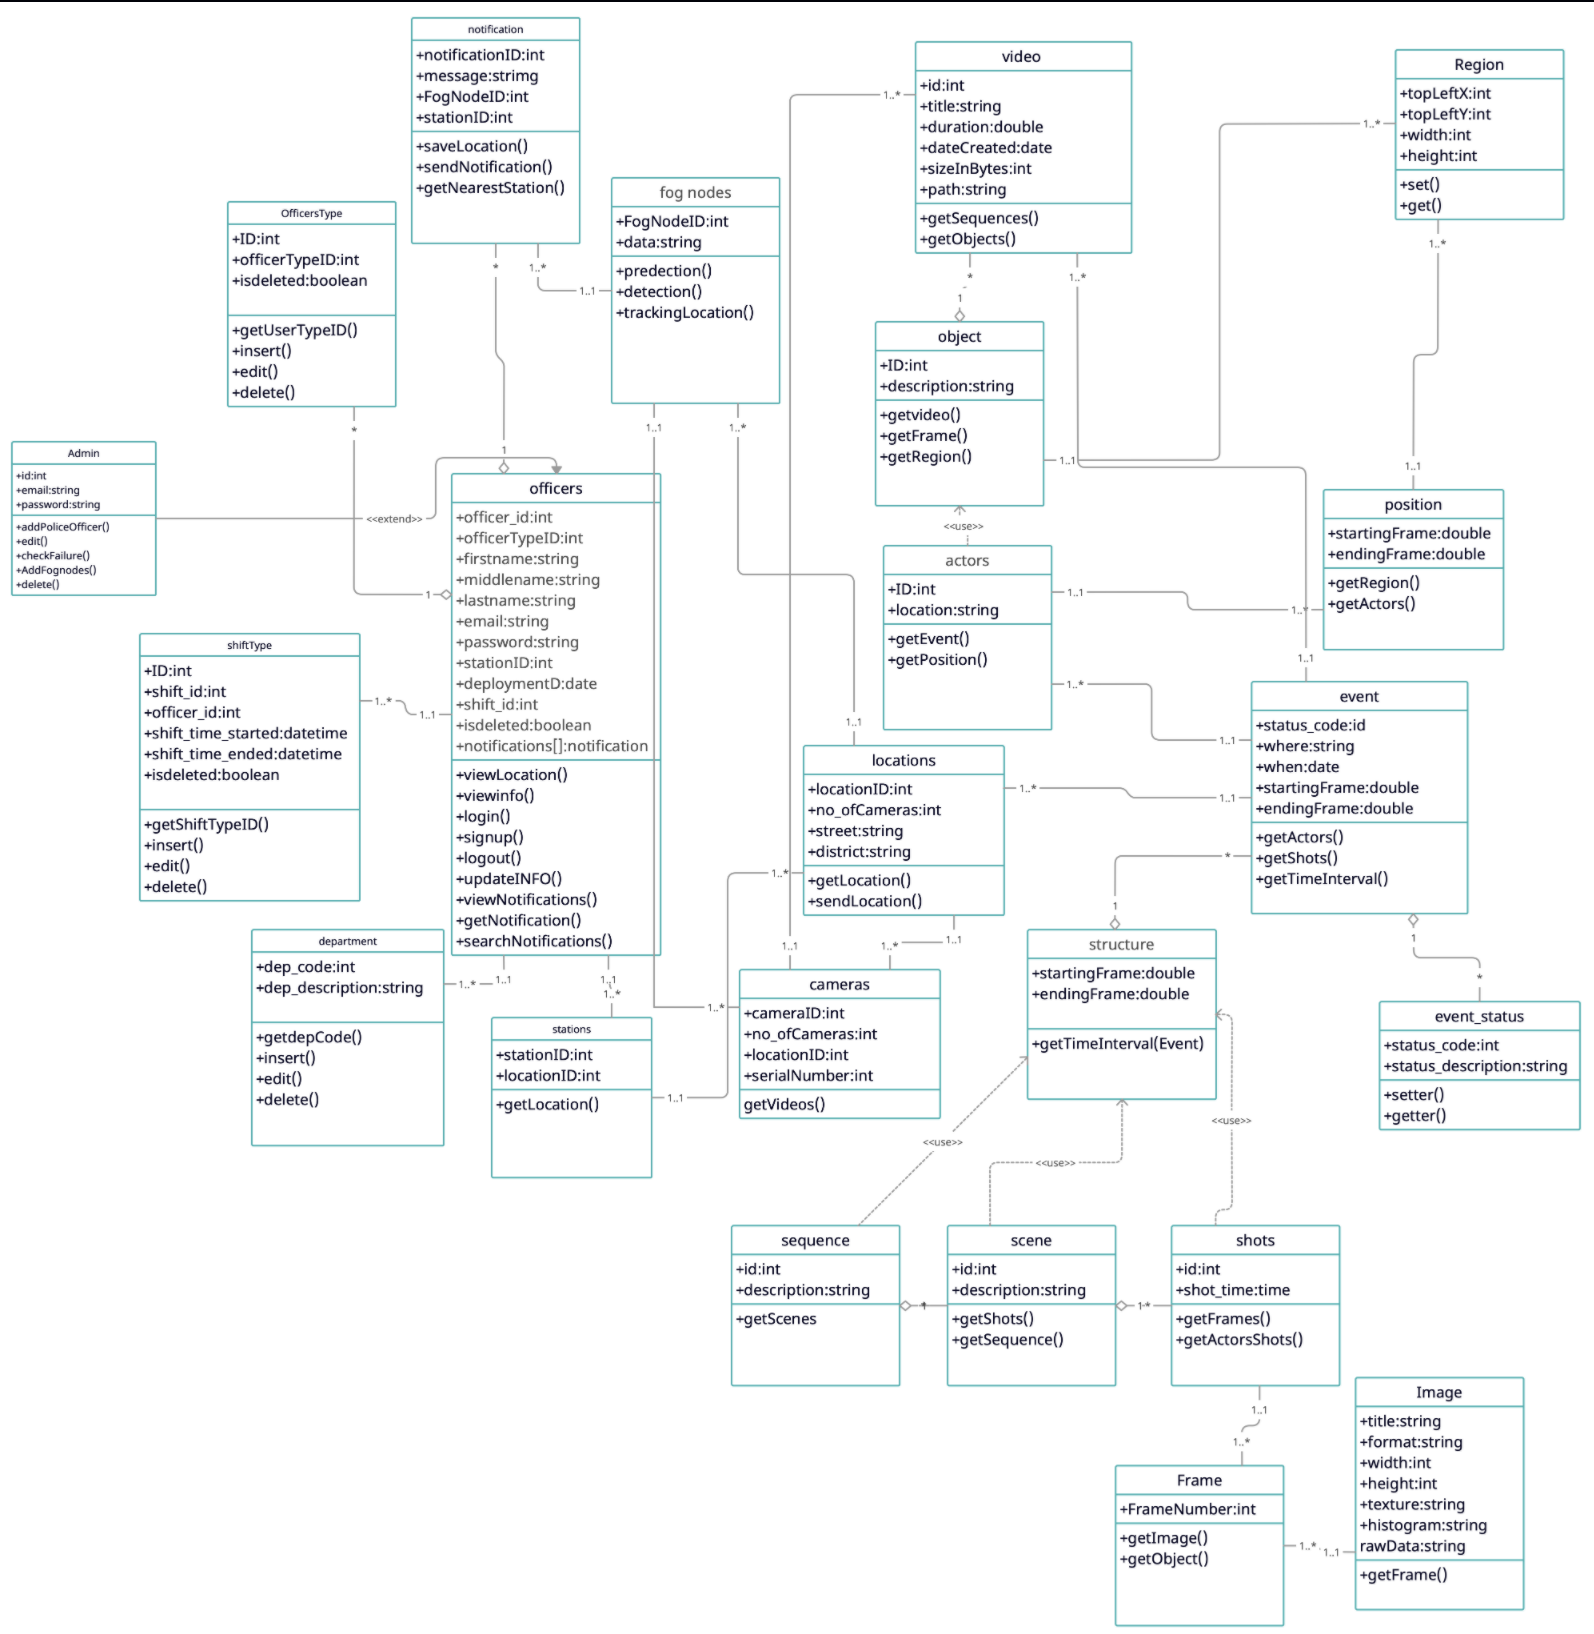
\includegraphics[width=0.85\linewidth]{classdiagram.png}
\caption{ClassDiagram }
\label{archdsgn}
\end{figure}
\subsubsection{Detailed classes}
\FloatBarrier

\begin{table}[h!]
\caption{Check failure of the camera}
\begin{tabular}{|p{0.15\textwidth}|p{0.85\textwidth}|}
\hline
\textbf{Name}           &  Check failure of the camera \\ \hline
\textbf{Code}           &  FR01 \\ \hline
\textbf{Priority}       & Extreme \\ \hline
\textbf{Critical}       & It's essential to detect if any failure happens to the video streams and enclose it to efficiently detect an event, avoid network overload, and improve the cloud storage usage \\ \hline
\textbf{Description}    & The system detects if any failure that impacts the usefulness of the video streams (i.e., natural occlusion, disruption) happens. Then, sending an alert of the failure to the maintenance team to recover it   \\ \hline
\textbf{Input}          & Video stream                                                                             \\ \hline
\textbf{Output}         & Boolean if it detects failure or not                                                                             \\ \hline
\textbf{Pre-condition}  & A failure happens in the video streams.                                                                                                                                                                    \\ \hline
\textbf{Post-condition} & A failure is detected and enclosed with an alert to the maintenance team to recover it      \\ \hline
\textbf{Dependency}     & -                                      \\ \hline
\textbf{Risk}           & - \\ \hline
\end{tabular}
\end{table} 
 \FloatBarrier
 \begin{table}[h!]
\caption{Crime detection}
\begin{tabular}{|p{0.15\textwidth}|p{0.85\textwidth}|}
\hline
\textbf{Name}           &  crime detection function \\ \hline
\textbf{Code}           & FR02 \\ \hline
\textbf{Priority}       & Extreme \\ \hline
\textbf{Critical}       & It is really essential; An action needs to be detected in order to take the appropriate action to predict or prevent it.   \\ \hline
\textbf{Description}    & It detects if an abnormal event occurs or everything is normal using a light-weighted CNN pre-trained model and forwards it. \\ \hline
\textbf{Input}          & video stream                                                                                                                                                                   \\ \hline
\textbf{Output}         &  video stream                                                                                                                                                                     \\ \hline
\textbf{Pre-condition}  & surveillance camera captures an event.                                                                                                                                                                    \\ \hline
\textbf{Post-condition} & the event gets detected.      \\ \hline
\textbf{Dependency}     & \begin{tabular}[c]{@{}l@{}}
FR01.\\ This function depends on FR01, because if any failure took place on surveillance \\ cameras, the event will not be detected.
\end{tabular}                                       \\ \hline
\textbf{Risk}           & If any failure happens when capturing video streams. \\ \hline
\end{tabular}
\end{table} 

 \FloatBarrier

\begin{table}[h!]
\caption{Face blurring}
\begin{tabular}{|p{0.15\textwidth}|p{0.85\textwidth}|}
\hline
\textbf{Name}           &  Face blurring \\ \hline
\textbf{Code}           & FR03 \\ \hline
\textbf{Priority}       & Extreme \\ \hline
\textbf{Critical}       & It's extremely essential to ensure the privacy and identity of the citizens that exposed to privacy violation in the video surveillance \\ \hline
\textbf{Description}    &In the real-time video surveillance after detecting the people's faces, the system uses a blur algorithm to blur the face to be indiscernible.  \\ \hline
\textbf{Input}          & Video stream                                           \\ \hline
\textbf{Output}         & Video stream                                             \\ \hline
\textbf{Pre-condition}  & Detecting people's faces in real-time video surveillance to blur it               \\ \hline
\textbf{Post-condition} &The detected faces are been blurred      \\ \hline
\textbf{Dependency}     & FR01 – FR02                                       \\ \hline
\textbf{Risk}           & If there is any failure that impacts the usefulness of the video stream \\ \hline
\end{tabular}
\end{table} 

\FloatBarrier
\begin{table}[h!]
\caption{Video Summarization}
\begin{tabular}{|p{0.15\textwidth}|p{0.85\textwidth}|}
\hline
\textbf{Name}           &  Video Summarization \\ \hline
\textbf{Code}           & FR04 \\ \hline
\textbf{Priority}       & Extreme \\ \hline
\textbf{Critical}       & It's extremely essential to ensure the incident and summarize the frames to the least possible and send them as images to help fast detection \\ \hline
\textbf{Description}    &In the real-time video surveillance after the edge nodes forwards a video stream with an incident, it must be trimmed into less frames video with only the incident part  \\ \hline
\textbf{Input}          & Video stream                       \\ \hline
\textbf{Output}         & Video frames as separate images      \\ \hline
\textbf{Pre-condition}  & Detecting an incident            \\ \hline
\textbf{Post-condition} &The detected incident is checked and summarized into some images with the parts of interest and forwards them. \\ \hline
\textbf{Dependency}     & FR01 – FR02                                       \\ \hline
\textbf{Risk}           & If there is any failure that impacts the usefulness of the video stream \\ \hline
\end{tabular}
\end{table} 
\FloatBarrier
\begin{table}[h!]
\caption{Final Crime classification}

\begin{tabular}{|p{0.15\textwidth}|p{0.85\textwidth}|}
\hline
\textbf{Name}           &   Crime classification \\ \hline
\textbf{Code}           & FR05 \\ \hline
\textbf{Priority}       & Extreme \\ \hline
\textbf{Critical}       & It's extremely essential to ensure the incident and classify them either fighting, robbery , kidnapping or it was wrongly detected to avoid false alarms \\ \hline
\textbf{Description}    & In the real-time video surveillance after the edge nodes forwards a video stream with an incident, and the fog nodes summarize them, the function ensure the incident and classify it and forwards it to FR06.\\ \hline
\textbf{Input}          & Video frame images                       \\ \hline
\textbf{Output}         & Video frames images with incident name and time    \\ \hline
\textbf{Pre-condition}  & Detecting an incident            \\ \hline
\textbf{Post-condition} &The detected incident is checked and summarized into some images with the parts of interest and forwarded to it. \\ \hline
\textbf{Dependency}     & FR01 – FR02 -FR04                                     \\ \hline
\textbf{Risk}           & If there is any failure that impacts the usefulness of the classifier or the images being processed \\ \hline
\end{tabular}
\end{table} 

\FloatBarrier
 
\begin{table}[h!]
\caption{Alert Function Description}
\begin{tabular}{|p{0.15\textwidth}|p{0.85\textwidth}|}
\hline
\textbf{Name}           & Alert  \\ \hline
\textbf{Code}           & FR06 \\ \hline
\textbf{Priority}       & Extreme  \\ \hline
\textbf{Critical}       & It is important to alert police by kidnapping incident. \\ \hline
\textbf{Description}    & To maintain the situation, there must an alert send to the police to come urgently and catch the criminal.. \\ \hline
\textbf{Input}          & Video frames , classified incident ,time,location                                               \\ \hline
\textbf{Output}         & Alert                             
\\ \hline
\textbf{Pre-condition}  & After detection of the incident in FR05 and face recognition in FR08, an alert must be sent to police by Fog computing.                      \\ \hline                                                                                     
\textbf{Post-condition} & Alert to police.      \\ \hline
\textbf{Dependency}     & 
FR05: By detection of the incident,  FR08: by Face recognition , Cloud will send an alert to the police to rescue the victim.FR08 to send the criminal face if possible
\\ \hline
\textbf{Risk}   & Failure to send an alert if there is data is missing or there was a difficulty to send an alert. \\ \hline
\end{tabular}
\end{table} 
 \FloatBarrier
\begin{table}[h!]
\caption{Face Recognition Function Description}
\begin{tabular}{|p{0.15\textwidth}|p{0.85\textwidth}|}
\hline
\textbf{Name}           & Face Recognition  \\ \hline
\textbf{Code}           & FR07 \\ \hline
\textbf{Priority}       & High  \\ \hline
\textbf{Critical}       & It is important to recognize the criminal's face to make it easy for the police to catch him. \\ \hline
\textbf{Description}    & After the crime is finally detected and classified the function in responsible for detecting the criminal's face if possible and send it to the camera's storage  \\ \hline
\textbf{Input}          & Video frame image                   \\ \hline
\textbf{Output}         & Criminal's face image              \\ \hline
\textbf{Pre-condition}  & the detection of an incident in FR05 \\ \hline                                  
\textbf{Post-condition} & Face recognition      \\ \hline
\textbf{Dependency}     & \begin{tabular}[c]{@{}l@{}}
FR05: the final detection of the incident and ensuring it.
\end{tabular}                                       \\ \hline
\textbf{Risk}           & Failure in camera when capturing criminal or the criminal is hiding his identity. \\ \hline
\end{tabular}
\end{table} 

 \FloatBarrier
\begin{table}[h!]
\caption{Compare Criminal Faces }
\begin{tabular}{|p{0.15\textwidth}|p{0.85\textwidth}|}
\hline
\textbf{Name}           & criminal Tracking Function \\ \hline
\textbf{Code}           &  FR08 \\ \hline
\textbf{Priority}       &  medium \\ \hline
\textbf{Critical}       & it is a supplementary function in the system to complete its functionalities \\ \hline
\textbf{Description}    & After detection of a crime incident their should be a tracking for the criminal by comparing his face with the data stored on the cameras after FR07 and check if he may be the wanted criminal. \\ \hline
\textbf{Input}          & video stream  \\ \hline
\textbf{Output}         & alert  \\ \hline
\textbf{Pre-condition}  & abnormal incident detected FR02,and video summarization in FR04 and Final classification FR05     \\ \hline
\textbf{Post-condition} & tracing kidnapper location and report the authorities \\ \hline
\textbf{Dependency}     & FR01-FR02-FR04-FR05 \\ \hline
\textbf{Risk}           & Camera has any failure in capturing the video streams and can be fixed with FR01, the incident couldn't be identified correctly,or his face can't be detected in FR07\\ \hline
\end{tabular}
\end{table} 

 \FloatBarrier
\subsection{Patterns use viewpoint}
This viewpoint addresses design ideas focusing on the used design patterns. 
UML class diagram and the UML package diagram can be used here to illustrate the used design patterns.
\subsubsection{Design Rationale}
You need to provide the design rationale for using these design patterns.

\subsection{Algorithm viewpoint}
The system consists of edge-fog layers, where each layer is responsible for a sequence of tasks that it completes and passes on to the next layer. 
\begin{itemize}
\item Sensors placed on street lights are introduced in this system as our edge nodes. The edge nodes are responsible for checking for camera failures. They make sure that the camera capturing is not interrupted quality-wise by any external sources. Moreover, edge nodes apply a human detection algorithm, as well as, face blurring to protect the privacy of the citizens. Also, a human intersection algorithm gets applied to acknowledge the meeting of two or more individuals. When this meeting occurs, the nodes determine the current location and send it, with the video streams, to the next layer. 
\item Vehicles are proposed as the system’s nodes for the second layer, the first tier fog layer. The fog nodes in this layer are responsible for applying feature extraction on video streams received by the edge layer, to decrease the computational power. Moreover, video summarization is applied to extract the most relevant information.
\item Summarized video streams are then passed to the second-tier fog layer, where the nodes are the traffic lights. Deep learning techniques are applied to determine if the contact between people was unproblematic or if an incident occurs. If an unusual event occurred, face detection gets carried out on the individuals, and a tracking algorithm is placed to track them.

\item The cloud layer, which is the last layer, collects all the data passed to it by the layers and triggers an alarm to police units.


\end{itemize}
\subsection{Interaction viewpoint}
\begin{figure}[h]
  \centering
  \includegraphics[width=19cm]{Activityy.jpeg}
  \label{fig:2}
   \caption{The workflow diagram of the framework}
\end{figure}


\subsection{Interface viewpoint}
\subsubsection{Main Page}
The admin can create accounts for multiple users. Each user logs into the system with his email and password. Moreover, each user can log out of the system.
\begin{itemize}
    \item Login allows the user to enter the system using his email and password
    \item Registeration allows the admin to create account for the users.
    \item Logout allows the user to exit the system.
\end{itemize}

\subsubsection{Location Page}
The location page consists of a map which views the incidents location. Users can track incidents to take appropriate action.

\subsubsection{Alert Page}
The alert page consists of alerts triggered by the cloud layer. It has all the information collected needed by police units to track and capture criminals.

\section{Data Design}
\subsection{Data Description}
Our system handles and processes data in various ways as data needed are retrieved from either the application implemented for storing users’ data or from the edge layer of our system’s architecture. Moreover, Data received from our dataset to train our models is originally in CSV file format. Data get captured in the application from the forms available for the users to fill in. On the other hand, sensors (cameras) placed on the edge layer capture data in video format to get processed further. Information extracted from users will be stored in Cloud Firestore, a NoSQL database that will provide our application with flexibility and scalability.


\subsection{Dataset Description}
We have acquired a data set of surveillance videos published by the \textbf{ 'UCF Center for research in computer vision'} called  \textbf{ UCF-Crime}; It is a large-scale dataset of 128 hours of videos; it has 1900 video of many classes as Robbery, Stealing, Shooting ... etc. And it is widely used in any research or project that targets public safety and surveillance. Therefore we took some of those videos from the classes that meet our requirements. \ref{tab:ds} illustrates the dataset.

\FloatBarrier
\begin{table}[htbp]
\centering
\label{tab:ds}
\caption{Dataset Description}
\begin{tabular}{ | l | m{11cm}|} 
\hline
\textbf{Dataset Name} & UCF-Crime Dataset   \\ 
\hline
\textbf{Link} &  https://www.crcv.ucf.edu/projects/real-world/ \\ 
\hline
\textbf{Size} & 95.9 GB  \\ 
\hline
\textbf{Number of classes} & The dataset has 13 classes for anomaly events and normal class; we used 3 of them  \\
\hline
\textbf{Average Video frames} & 1000-1500 frames per video \\
\hline
\textbf{Number of videos used} & we used for fighting 10 videos,Robbery 10 videos,normal events 10 videos \\
\hline
\textbf{comments} & This data set has many videos in many places; we chose the suitable videos in streets. Also it didn't include kidnapping events; so we gathered 6 surveillance videos from Youtube with same video length and specifications as UCF-crime videos \\
\hline
\end{tabular}
\end{table}
 \FloatBarrier
\begin{figure}[h]
  \centering
  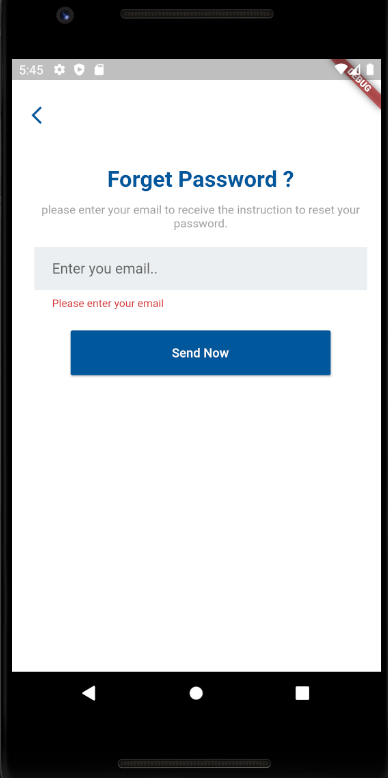
\includegraphics[width=5cm]{ForgetPass.PNG}
  \label{fig:2}
   \caption{Forget Password}
\end{figure}
\FloatBarrier
\begin{figure}[h]
  \centering
  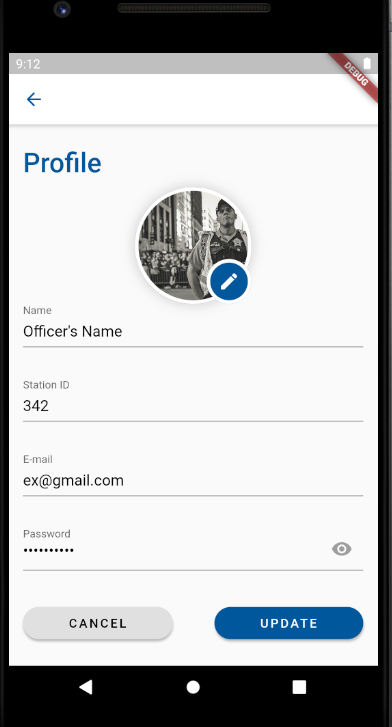
\includegraphics[width=5cm]{profile.PNG}
  \label{fig:2}
   \caption{Profile}
\end{figure}
\FloatBarrier
\begin{figure}[h]
  \centering
  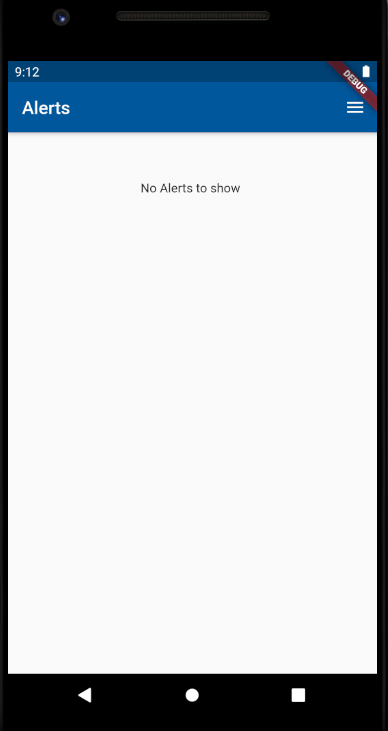
\includegraphics[width=5cm]{Alerts.PNG}
  \label{fig:2}
   \caption{Alerts Page}
\end{figure}
\FloatBarrier
\begin{figure}[h]
  \centering
  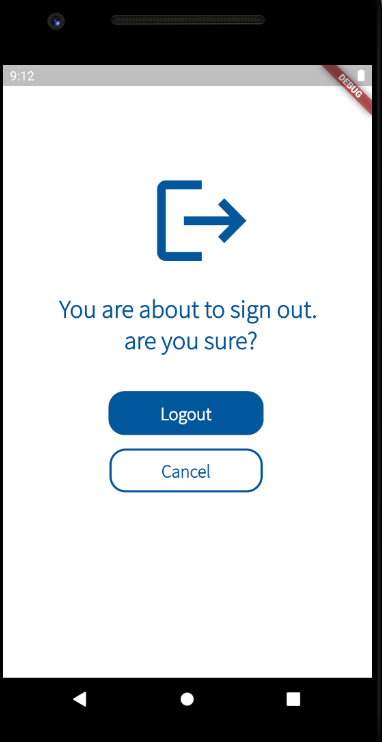
\includegraphics[width=5cm]{Logout.PNG}
  \label{fig:2}
   \caption{Logout Page}
\end{figure}

\subsection{Database design description}
Describe any databases (provide database schema diagram) and/or description of other data storage items.

\section{Human Interface Design}
\label{hid}
\subsection {User Interface}
The proposed system's application focuses on two main ends. User end and admin end. The application allows the admin to login and creates accounts for the police officer or security guards. Also, the admin can update and delete the user's account. The user will log in to the application with an email and password set by the admin. Also, the user can update his information and change his password. Moreover, the user will view the alerts sent by the system with images, location, and time.

Admin: Admin will log in through the application login page. Admin can add accounts by filling the fields in add account page with proper information.

User: The user will log in through the application login page. He will be able to edit the profile by updating the user's info through the profile page. Also, the user will view the alerts sent by the system with their details on the alert page.

\subsection {Screen Images}
\FloatBarrier
\begin{figure}[h]
  \centering
  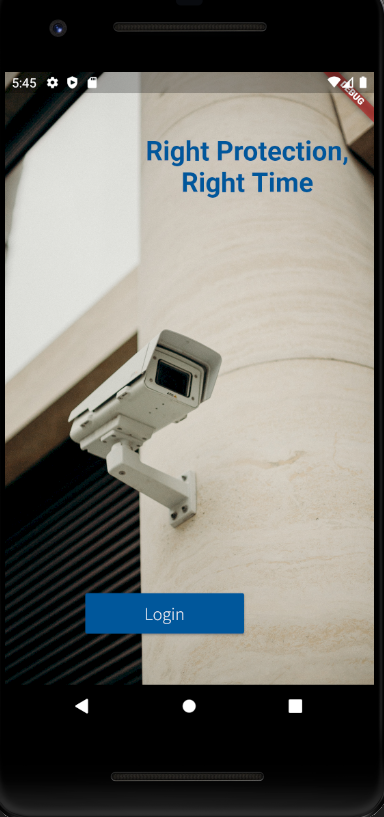
\includegraphics[width=5cm]{HomePage.PNG}
  \label{fig:2}
   \caption{Home Page}
\end{figure}
\FloatBarrier
\begin{figure}[h]
  \centering
  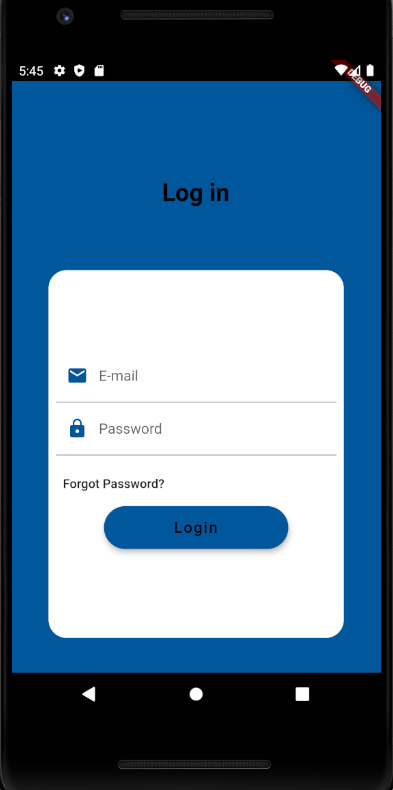
\includegraphics[width=5cm]{Login.PNG}
  \label{fig:2}
   \caption{Login Page}
\end{figure}
\FloatBarrier
\begin{figure}[h]
  \centering
  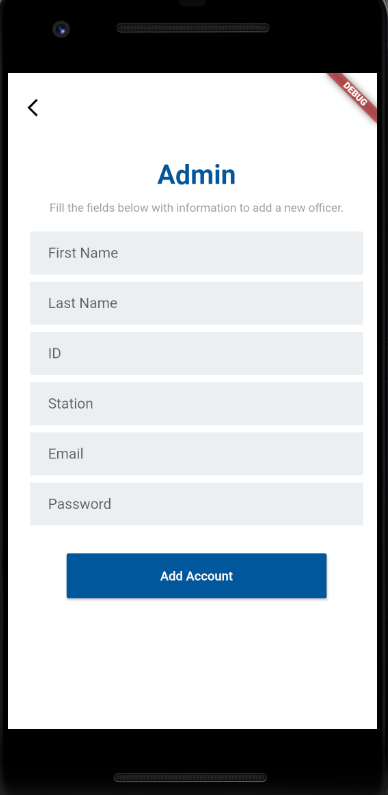
\includegraphics[width=5cm]{AddAccount.PNG}
  \label{fig:2}
   \caption{Add new account}
\end{figure}

\subsection {Screen Objects and Actions}
A discussion of screen objects and actions associated with those objects.

\section{Requirements Matrix}
Provide a cross reference that traces components and data structures to the requirements in your SRS document.
Use  a  tabular  format to show  which system  components satisfy each of the  functional 
requirements from the SRS. Refer to the functional requirements by the numbers/codes that you gave them in the SRS as shown in Table \ref{tab:RM}.

\begin{table}[htbp]
\centering
\caption{Requirements Ratrix}
\label{tab:RM}
\begin{tabular}{|l|l|l|l|l|}
\hline
Req. ID  & Req Desc & Class & Test Cases ID & Status      \\ \hline
FR01     & xxxx     & class name & TC01, TC02    & In Progress \\ \hline
FR02     & xxxx     & class name & TC03, TC04    & Developed   \\ \hline
\end{tabular}
\end{table}

\section{APPENDICES}
Appendices may be included, either directly or by reference, to provide supporting details that could aid in the understanding of the Software Design Document.
\subsection{Github}
Add screenshots from Github repository showing your project.

\subsection{ Other appendices as appropriate}
Optional section.

\printbibliography

\end{document}
